\section{Limit Definition}
\begin{definition}
	Let $f : D \subseteq \R \to \R$.
	Let $c \in R$ be a limit point (ie $c \in D$ or $c$ is on the boundary of $D$).
	$f$ has a limit $L$ as $x$ approaches $c$ if for any given positive real number $\epsilon$, there is a positive real number $\delta$ such that for all $x \in D$,
	\begin{equation}
		0 < \abs{x-c} < \delta \implies \abs{f(x) - L} < \epsilon.
	\end{equation}
	We write this as
	\begin{equation*}
		\lim_{x \to c}{f(x)} = L.
	\end{equation*}
\end{definition}

\begin{figure}[H]
	\label{epsilon_delta}
	\centering
	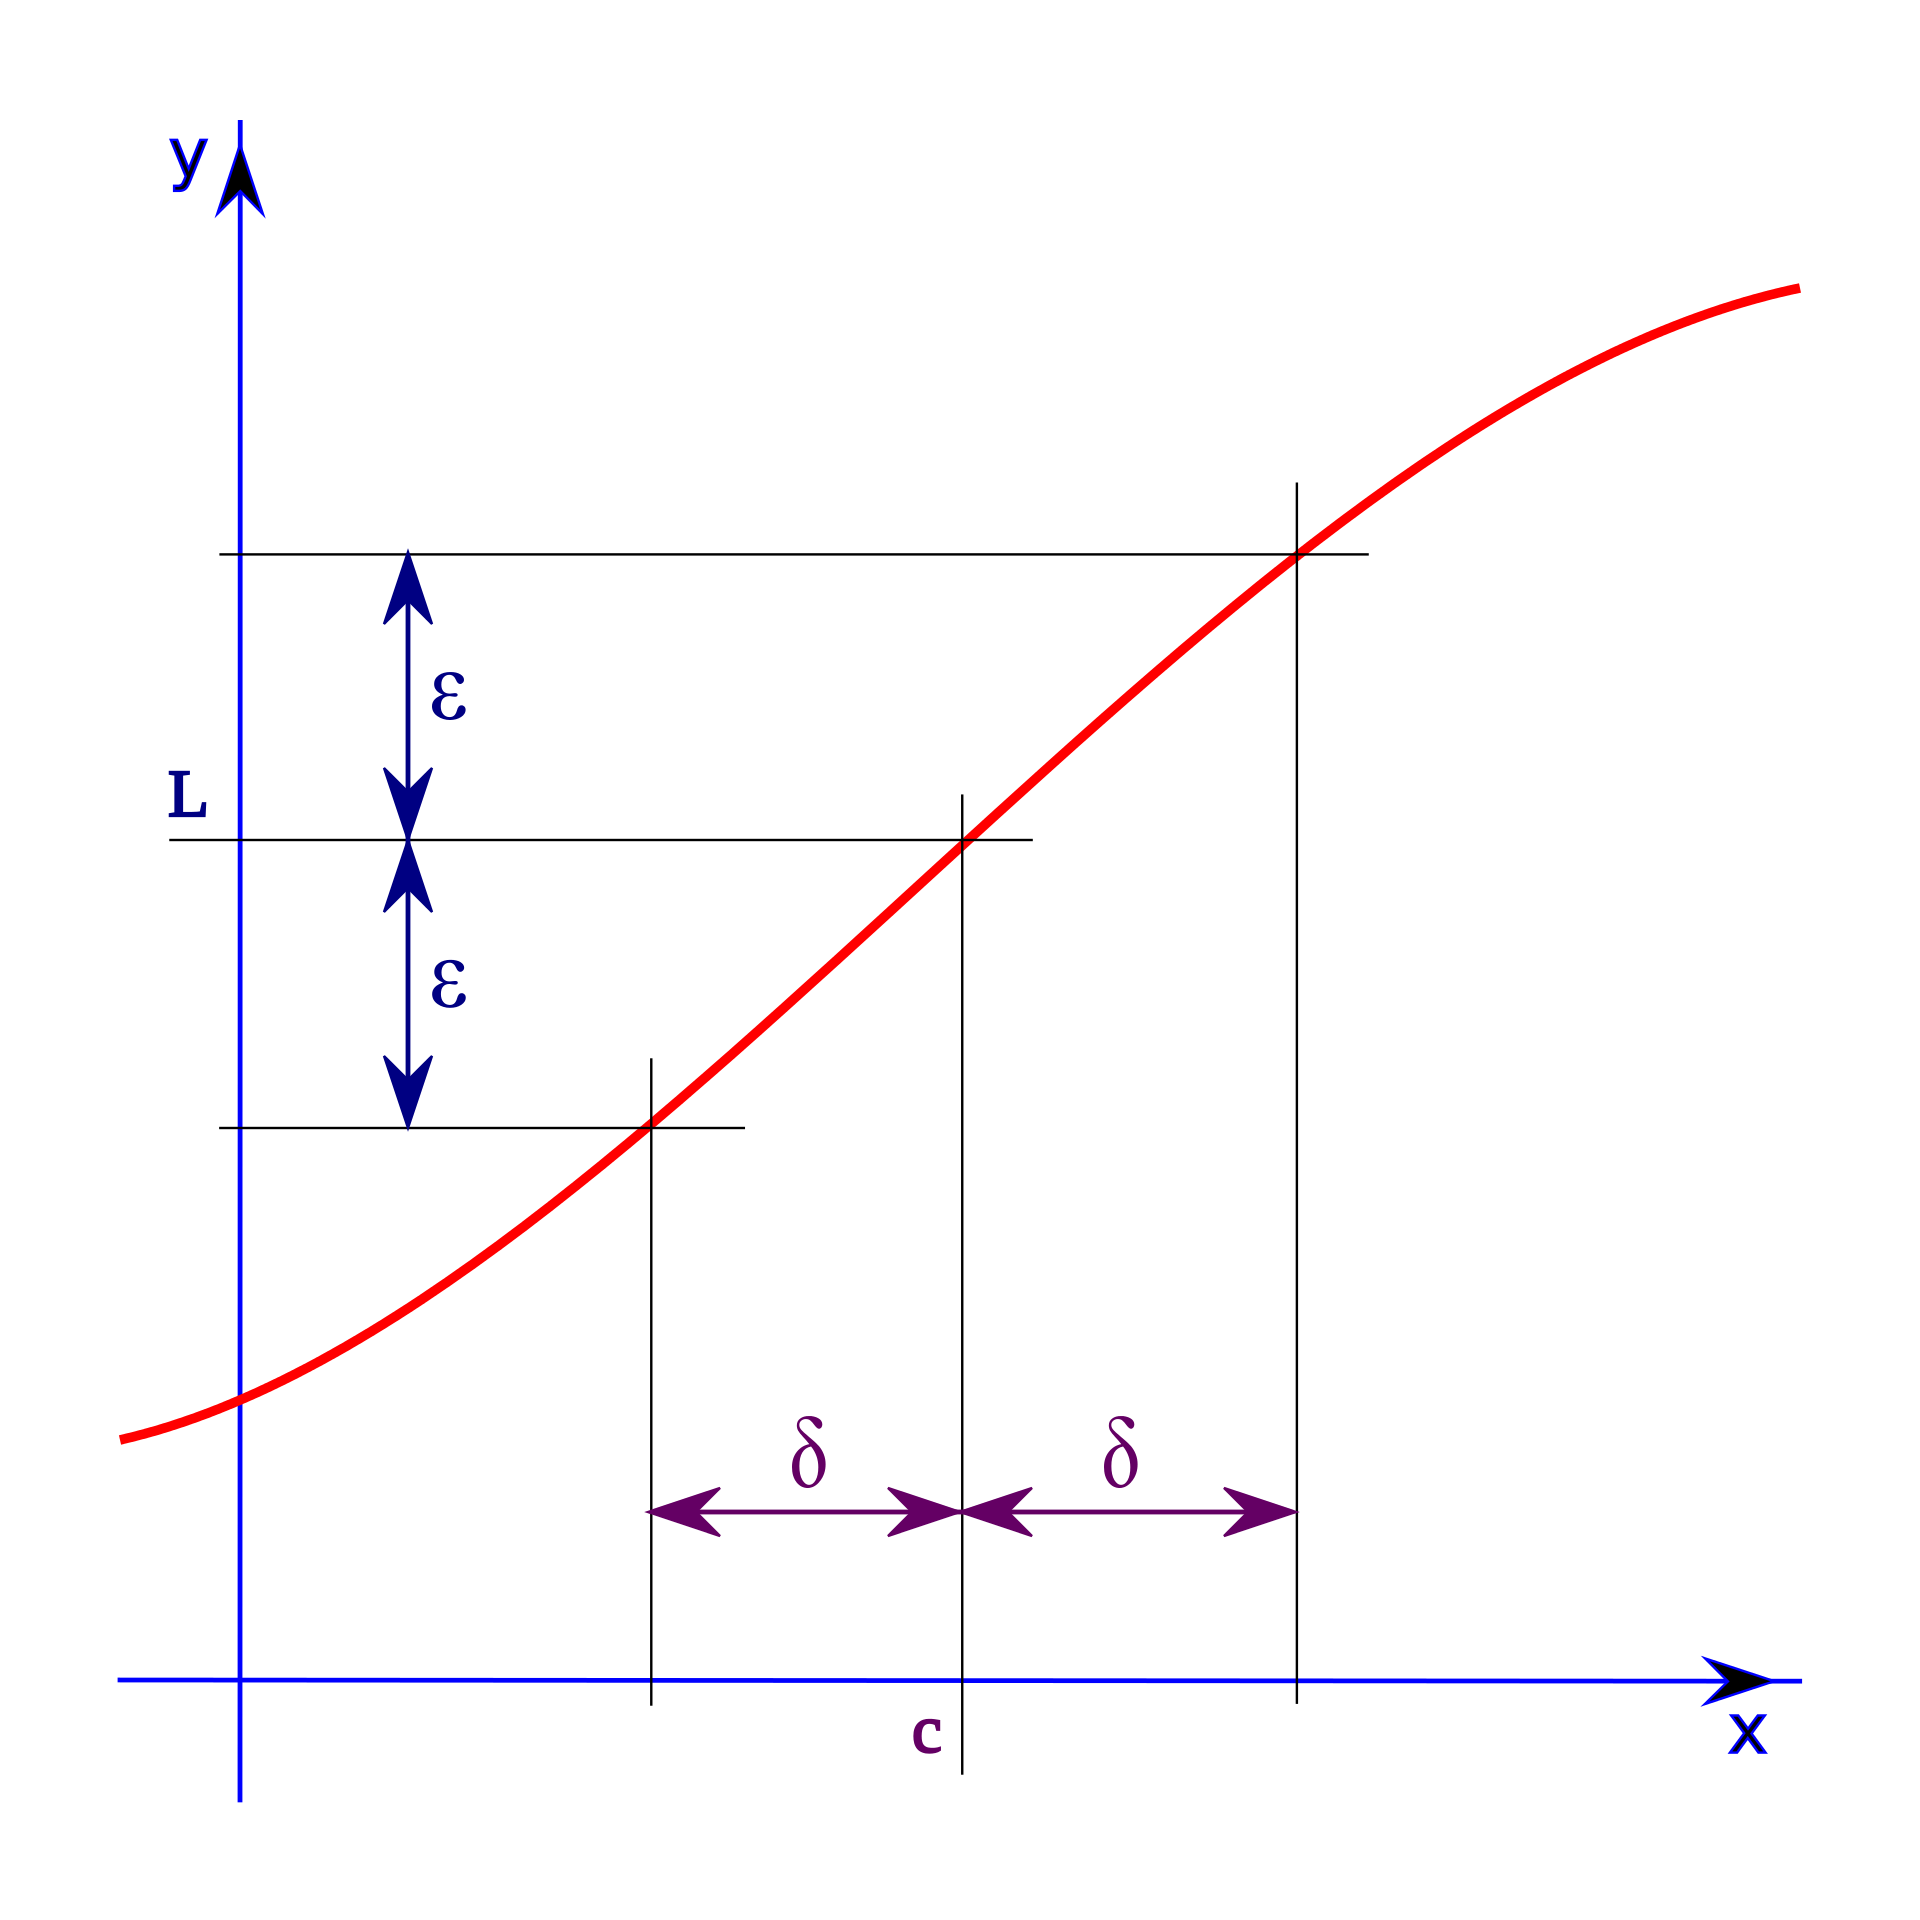
\includegraphics[width = 0.5\textwidth]{./limits_continuity/limit_epsilon_delta.png}
	\caption{\hyperref{https://en.wikipedia.org/wiki/(\%CE\%B5,\_\%CE\%B4)-definition\_of\_limit}{}{}{Wikipedia - $(\epsilon, \delta)\text{-definition of limit}$}}
\end{figure}

Visually, what this means is that for any "error bound" of $y$ values $\epsilon$, I can give you a corresponding error bound of $x$ values $\delta$ such that all values of $f(z)$ for $z \in (c -\delta, c+ \delta)$ bound are between $L - \epsilon$ and $L + \epsilon$.


We don't use this definition of the limit very often because it's a bit cumbersome.
However, it's important to know that when we use the limit, this is the formal definition making things work.

\begin{example}
	Use the $(\epsilon, \delta)$ definition of the limit to show that
	\begin{equation*}
		\lim_{x\to 0}{x\sin{\frac{1}{x}}} = 0.
	\end{equation*}
\end{example}
\begin{answer}
	Letting $\epsilon > 0$, we need to find corresponding $\delta > 0$ that satisfies the definition for $L = 0$.
	Knowing that $\sin$ is bounded between -1 and 1,
	\begin{equation*}
		\abs{x\sin{\frac{1}{x}} - 0} = \abs{x\sin{\frac{1}{x}}} = \abs{x}\abs{\sin{\frac{1}{x}}} \leq \abs{x}.
	\end{equation*}
	
	Letting $\delta = \epsilon$, if $0 < \abs{x - 0} < delta$, then $\abs{x\sin{\frac{1}{x}} - 0} \leq \abs{x} < \epsilon$, as required by the definition.
\end{answer}